\documentclass[9pt]{beamer}
\usefonttheme[onlymath]{serif}
\usepackage[sfdefault]{roboto}
\usepackage[utf8]{inputenc}
\usepackage[T1]{fontenc}
\usepackage{styles/fluxmacros} 	% Define where theme files are located. 
\usefolder{styles}
\usetheme[style=red]{flux} % Available styles: asphalt, blue, red, green, gray 



\usepackage{graphicx}
\usepackage{amsmath}
\usepackage{amssymb}
\usepackage{amsfonts}

\title{Computerpraktikum Algebra}
\subtitle{Thema 4 - Graphen und Lie-Algebren}
\author{Pascal Bauer, Raphael Millon, Florian Haas}
\institute{Sommersemester 2020}
\date{\today}
\titlegraphic{assets/Empty.png}

\begin{document}

\titlepage 

\begin{frame}
 \frametitle{Table of contents}
 \tableofcontents
\end{frame}

\section{Theorie}
\begin{frame}{Theorie}
\begin{itemize}
\item Wir betrachten Dynkin-Diagramme und die daraus konstuierbaren Gruppen.
\item Dynkin-Diagramm sind spezielle Graphen, mit eventuell mehrfachen gerichteten Kanten.
\end{itemize}
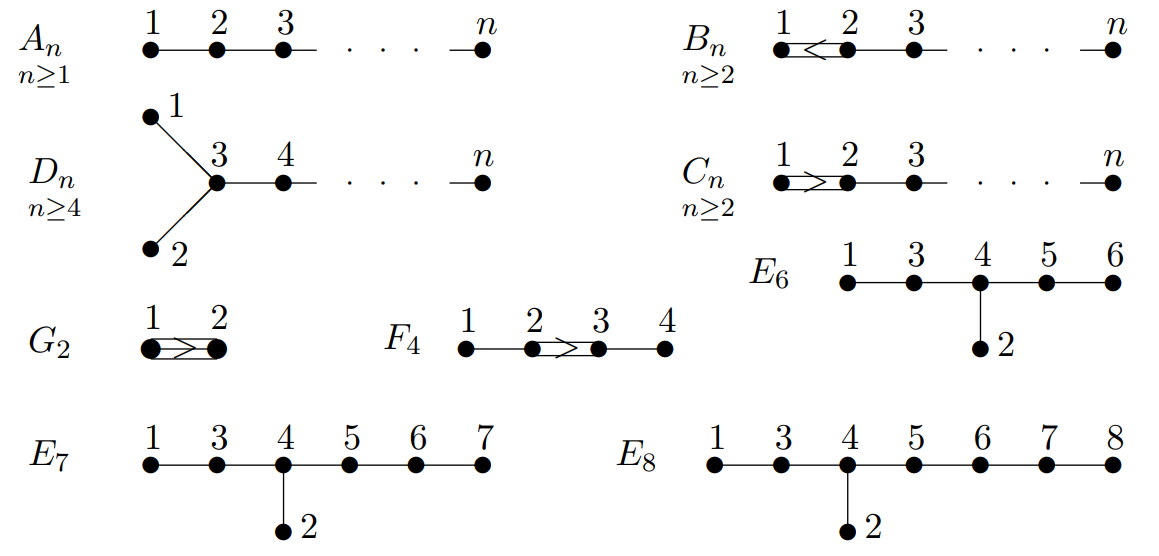
\includegraphics[width=\textwidth]{assets/dynkin.png}
\end{frame}

\begin{frame}{Theorie}
\begin{itemize}
\item Zu einem Graphen $\Gamma$ kann eine Matrix $A(\Gamma)=(a_{ij})_{1\leq i,j \leq n}$ wie folgt definiert werden:
\item \begin{enumerate}
	\item Setze $a_{ii} = 2$ auf der gesamten Diagonalen.
	\item Setze $a_{ij} = 0$, falls $i \neq j$ und die Ecken $i$ und $j$ nicht verbunden sind.
	\item Setze $a_{ij} = a_{ji} = -1$, falls $i \neq j$ und die Ecken $i$ und $j$ einfach verbunden sind.
	\item Setze $a_{ij} = -d, \ a_{ji} = -1$, falls $i \neq j$ und die Ecken $i$ und $j$ $d$-fach in Richtung $i$ verbunden sind.
	\end{enumerate}
\item Für $F_4$ ergibt sich zum Beispiel $$A(F_4)=\begin{pmatrix}2&-1&0&0\\-1&2&-1&0\\0&-2&2&-1\\0&0&-1&2\end{pmatrix}.$$
\item Somit kodieren sich $\Gamma$ und $A(\Gamma)$ gegenseitig.
\end{itemize}
\end{frame}

\begin{frame}{Theorie}
\begin{itemize}
\item Für festes $\Gamma$ definieren wir nun für $1 \leq i \leq n$ lineare Abbildungen gegeben durch $w_i(e_j) := e_j - a_{ij}e_i$ oder äquivalent $M_{\mathbb Q}(w_i) = I_n - E_{ii}A(\Gamma)$.
\item Da $M_{\mathbb Q}(w_i)^2 = I_n - 2E_{ii}A(\Gamma) + (E_{ii}A(\Gamma))^2 = I_n$ ist die Abbildung $w_i \in GL_n(\mathbb Q)$ und insbesondere diagonalisierbar mit Eigenwerten $\in \{-1,1\}$.
\item Jede Abbildung $w_i$ beschreibt also eine Spiegelung.
\item In unserem Projekt betrachteten wir die von allen $w_i$ erzeugte Gruppe $W = \langle w_1, \ldots, w_n \rangle \subseteq GL_n(\mathbb Q)$.
\item Zudem wird $\Phi = \{w(e_j) \mid w \in W, 1 \leq j \leq n\}$ berechnet. Insbesondere ist $\Phi$ genau dann endlich wenn auch $W$ endlich ist.
\end{itemize}
\end{frame}



\section{Showcase}
\begin{frame}{Showcase}
gmat\\
glin\\
gphi\\
\end{frame}
\section{Ausgesuchte Codebeispiele}
\begin{frame}{Codebeispiele}
GAP GAP GAP
\end{frame}
\end{document}